\chapter{PEG \& CFG Semantics}
\label{chap:peg_cfg_semantics}

\section{Recap}
    \theoremstyle{definition}
    \begin{definition}[Grammar]
        The (formal) definition of a language
    \end{definition}
    \theoremstyle{definition}
    \begin{definition}[Language]
        A (potentially infinite) set of sentences
    \end{definition}
    \theoremstyle{definition}
    \begin{definition}[Parser]
        Recognizes a sentence in the language + extract a syntax tree
    \end{definition}
    \theoremstyle{definition}
    \begin{definition}[Parsing Tool]
        Generate and/or runs parsers
    \end{definition}
    Two types of formalism : 
    \begin{itemize}
        \item CFG (Context-Free-Grammar)
        \item PEF (Parsing Expression Grammar)
    \end{itemize}
    Notations : 
        \begin{itemize}
            \item (E)BNF (usually for CFG)
            \item PEG Notation (usually for PEG)
        \end{itemize}
    \theoremstyle{definition}
    \begin{definition}[Non-Terminal]
        Things that we define
    \end{definition}
    \theoremstyle{definition}
    \begin{definition}[Terminals]
        Tokens, strings, etc. that cannot be extended further.
    \end{definition}

\section{Context-Free Grammars}
    Usually a CFG is defined as a tuple of 4 components Grammar = $(N, \Sigma, P, S)$: 
        \begin{itemize}
            \item N: Non-Terminals
            \item $\Sigma$: Alphabet (Terminals)
            \item P: Production Rules ($P: N \rightarrow (\Sigma \cup N)*$)
            \item Starting Symbol ($S \in N$)
        \end{itemize}

    In order to have a CFG from a "full" grammar, we first need to replace all
    syntactic sugars by the complete recursive rules, then eliminate all choices
    by introducing as many rules as we have choices.

    \subsection{Semantics Derivation}
        \begin{itemize}
            \item The language defined by a CFG is the set of all sentences that
            can be derived from its rules
            \item Start from the start symbol, replace it by the right-hand side
            of one its production
            \item At each step, replace a non-terminal from the current string
            symbol by its definition (until no non-terminals are left in the string)
            \item Any terminal, the order does not matter
        \end{itemize}
        Note that by doing that, we define the language, not a parsing algorithm
        and we're doing it in a generative way grammar $\rightarrow$ sentences.

        Also, if we would have used characters derivation instead of tokens we
        would have need to continue to derive which would of potentially lead to
        an infinite derivation. So, we can say that for a sentence to be part of
        a language in need to be derivable however we cannot describe the all
        derivation table because in many case, it would be infinite.
\section{PEG Semantics}
    We can see in the slide (9 of PEG - CFG semantics's pdf) the use of a
    top-down recursive descent parsers that produce production rules (with
    lookahead operator as an exception).

\section{PEG vs CFG}
    \subsection{Semantics}
        CFG are generative (their semantics is given by constructing the language
        set by the grammar through derivation). On the other hand PEG are
        recognition based : a sentence is in the language defined by a PEG grammar
        only if it is recognized by the language recognizer. In order to formalize
        PEG grammar we need to formalize the recognizer for the grammar.

        These two approaches are very different in the mathematical point of view.
        Also, CFG is easier to defined in the mathematical language, on the other
        hand the PEG is very much related to the practice.
    \subsection{PEG vs CFG}
        \begin{itemize}
            \item CFG has unordered choices, while derivating we can pick any
            non-terminal we want
            \item PEG has ordered choices, the first matching is the "correct"
            one
        \end{itemize}
    \subsection{The differences}
        Unordered and ordered has a consequence for parsing algorithm. PEG does
        not test anything after a fail (prefix capture) if the parse failed
        while CFG can make an other choice!
        \subsubsection{PEG: Single parse Rule}
            Once a choice have been made, we never visit it again. As repetition
            can be desugared to choice it has an impact on them too. Repetition
            are greedy. (A ::= a* a is empty as a* will consume everything).
        \subsubsection{Backtracking}
            Let's take the following grammar : 
            \begin{itemize}
                \item A ::= B y z
                \item B ::= v | x y | x
                \item input: "xyz"
            \end{itemize}
            \begin{figure}[H]
                \centering
                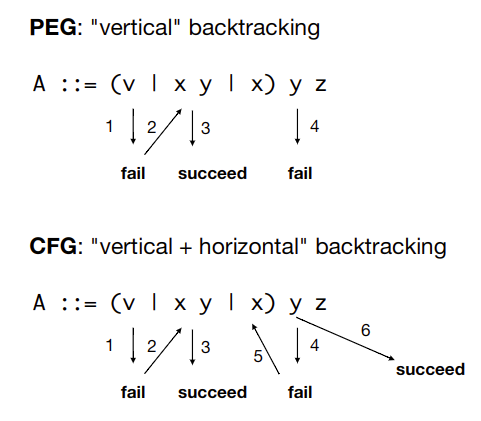
\includegraphics[scale=0.3]{PEG_CFG_BA.png}
                \caption{PEG vs CFG backtracking}
                \label{fig:peg_cfg_backtrack}
            \end{figure}
            This is not the real working way, be it does illustrate the
            principle. Indeed doing that would lead to exponential time
            complexity. CFG has horizontal backtracking thanks to is possibility
            to backtrack on x after trying y.
        \subsubsection{Ambiguity}
            It seems that CFG are always better because of what we have seen
            before. However there is a flip-side : ambiguity. By construction
            PEG cannot suffer from ambiguity.
            
            As a remainder : 
            \begin{itemize}
                \item Prefix capture (The rule B will consume all y)
                \begin{itemize}
                    \item A ::= B y z
                    \item B ::= x y | z
                \end{itemize} 
                \item Ambiguity (B can be xy or x, C can be z or yz): 
                \begin{itemize}
                    \item A ::= B C
                    \item B ::= x y | x
                    \item C ::= z | yz
                \end{itemize}
            \end{itemize}
            Ambiguity make the AST creation harder and also has impact on the
            parser performances.
        \subsubsection{Performances}
            The best parsing algorithm for CFG are $\mathcal{O}(n^3)$,
            deterministic parts of the grammar run in $\mathcal{O}(n)$ (most of
            useful grammar are deterministic).
            
            For PEGs, the regular algorithm is exponential (in theory). Still,
            it is almost impossible to write an $ \mathcal{O}(x^n)$ exponential
            parser. However, one often use operation is very inefficient : infix.

            An example can be this one : 
            \begin{itemize}
                \item S ::= P '+' S | P '-' S | P
                \item P ::= N '*' P | N '/' P | N
                \item N ::= [0-9]+
            \end{itemize}
            (Note that PEG does not allow left recursion by definition.) Let's
            assume we have a parseN function, if we try to parse "42", parse N
            will be called 9 times! 3 times for P, 3 times for S, 3x3=9. In
            general : $\mathcal{O}((P+1)^L)$ times with L : precedence levels (2
            here), P : operators at each level (3 here). 

            A solution for that can be found, for example in Autumn we can write : 
            \begin{lstlisting}[language=Java]
                rule P = left_expression()
                            .operand(N)
                            .operand('*')
                            .operand('/'); //Same for S however, operand is P in S, for precedence
            \end{lstlisting}
            This rewrite the grammar as : 
            \begin{itemize}
                \item S ::= P ( '+' S | '-' S)*
                \item P ::= N ( '*' P | '/' P)*
                \item N ::= [0-9]+
            \end{itemize}
            P and N will be only called once! Performances are good thanks to
            that! However we can note that the parse tree won't be nice (not a
            problem with Autumn as we build an AST explicitly (we give a
            function to create the nodes)). If we were not using Autumn, we
            should create the parse tree like that and then, rewrite it

            \paragraph{Packrat Parsers}
                The single parser rule make memoization very easy! Packrat
                Parser are PEG parser with memoization. However, some practical
                experiments have been done in Java shown it is slower. Unless
                maybe if your language is very slow, or unless your infix
                expressions are improperly implemented.
        \subsubsection{Expressivness}
            \begin{itemize}
                \item Some PEGs definition cannot be defined with CFG ( A ::=
                $a^n b^n c^n$ for any same n we want any a b c)
                \item Some CFGs definition cannot be defined with PEGs (A ::= a
                A a | b A b | a | b | $\epsilon$)
                \item Traditional PEG can't use left recursion (use repetition
                or Autumn to solve that, as they are the only two big case where
                we need left recursion)
            \end{itemize}
        \subsubsection{PEG : Lookahead operators}
            \begin{itemize}
                \item \&<expression>, succeeds if the expression succeeds but
                does not consume any input
                \item !<expression>, succeeds if the expression fails, does not
                consume any input
                \item In theory, \&X == !!X (not true in Autumn)
            \end{itemize}
        \subsubsection{PEG misc}
            PEGs are often use in scannerless parsing (without lexer), ordered
            and lookahead are very useful at lexical level. PEG allow us to
            define "reserved works", hence lexing can still be advantageous.

            PEGs are easy to extends thanks to recursive descent (with new
            combinators).
\section{Summary}
    PEG : 
        \begin{itemize}
            \item Intentional language = sentences recognized
            \item Similar to handwritten top down recursive descent parsers
            \item Desugared to CFG + lookahead
            \item Single parse rule
            \item Suffer from prefix capture
            \item Vertical backtracking
            \item Deterministic
            \item Ordered
            \item Potentially exponential, in practice largely linear (careful
            with infix)
        \end{itemize}
    CFG : 
        \begin{itemize}
            \item Extensional language = set of sentences obtained by derivation
            \item Suffer from ambiguity
            \item Vertical and horizontal backtracking
            \item Non deterministic
            \item Unordered
            \item $\mathcal{O}(n^3)$ but often linear in practice
        \end{itemize}
    In the end, both formalisms are good enough, the real difference is tooling,
    what is available in the language we want to use, ease of use, features,
    performances, etc.
            